\documentclass{ctexart}                             % 文档类型为article

\usepackage{geometry}                               % 引入geometry宏包
\geometry{a4paper, scale = 0.80}                    % 定义纸张和版面缩放
\usepackage{hyperref}                               % 引入hyperref宏包,实现跳转
\usepackage{amsmath, amssymb, amsthm, mathtools}    % 引入常用的数学宏包
\usepackage{tikz}                                   % 引入tikz宏包,用于绘图
\usepackage{siunitx}                                % 引入国际单位制宏包
\usepackage{xcolor}                                 % 引入用于定义颜色的宏包
\definecolor{LightBlue}{RGB}{226, 247, 254}         % 定义颜色 LightBlue
\definecolor{SierraBlue}{RGB}{192 ,207, 222}        % 定义颜色 SierraBlue
\usepackage{comment}                                % 引入注释宏包
\usepackage{tcolorbox}                              % 引入tcolorbox宏包
\tcbuselibrary{breakable, most, skins, theorems}    % 调用 tcolorbox 的相关功能
\newtcolorbox{question}[2][breakable] {             % 定义 [题目] 的样式
    colback = LightBlue,                            % 定义 填充色为LightBlue
    colframe = cyan,                                % 定义 边框颜色是cyan青色
    fonttitle = \bfseries,                          % 定义 题目编号的字体
    title = #2, #1                                  % 定义 题目编号依次从参数#2 #1传入
}
\newenvironment{solution} {
    \noindent{\textbf{{\color{cyan}解答}}}\quad     % 手动用新环境定义一套 [解答] 样式
}

%%%%%%%%%%%%%%%%%%%%%%%%%%%%%%%%%%%%%%%%%%%%%%%%%%%%%%%%%%%%%%%%%%%%%%%%%%%%%%%%%%%%
% 如何输入不同层级的标题?
% \section{一级标题}
% \subsection{二级标题}
% \subsubsection{三级标题}
% 
% 
% 如何编辑 [题目] ?
% 具体的样式定义在文件头部: \newtcolorbox{question}
% \begin{question}{题目编号(必填)}
%     这里输入详细的题目
% \end{question}
% 
% 
% 如何编辑 [解答] ?
% 具体的样式定义在文件头部: \newenvironment{solution}
% \begin{solution}
%     这里输入详细的解答过程
% \end{solution}
% 
% 
% 如何表示物理单位?
% 需要在文件头部引入siunitx宏包
% \,\si{这里填写单位}
%%%%%%%%%%%%%%%%%%%%%%%%%%%%%%%%%%%%%%%%%%%%%%%%%%%%%%%%%%%%%%%%%%%%%%%%%%%%%%%%%%%%


% \excludecomment{solution} % 编译这条指令会隐藏所有解答,生成习题册

\begin{document}

\title{《热学》部分课后习题解答}
\author{郭文锑}
\maketitle

\tableofcontents

\section{导论}

\begin{question}{题目1.3.2}
    定体气体温度计的测温泡浸在水的三相点槽内时,其中气体的压强为$6.7\times10^3\,\si{Pa}$.
    \begin{enumerate}
        \item[(1)] 用温度计测量 $300\,\si{K}$ 的温度时,气体的压强是多少?
        \item[(2)] 当气体的压强为 $9.1\times 10^3\,\si{Pa}$ 时,待测温度是多少?
    \end{enumerate}
\end{question}

\begin{solution}
    (1) 温度计在初始状态下的内部压强为 $p_1$ ,温度为 $T_1 = 273.15 \si{K}$,根据物态方程 $pV = \nu RT$ 有
    $$
        p_1 = \frac{\nu RT_1}{V} = 6.7 \times 10^3 \,\si{Pa}
    $$
    当温度计在测量 $T_2 = 300\,\si{K}$ 时,内部压强变为
    $$
        p_2 = \frac{\nu RT_2}{V}
        = \frac{p_1}{T_1}T_2
        \approx 7.4 \times 10^3 \,\si{Pa}
    $$
    (2) 温度计在初始状态下的内部压强为 $p_1$ ,温度为 $T_1 = 273.15 \si{K}$ ,根据物态方程 $pV = \nu RT$ 有
    $$
        T_1 = \frac{p_1V}{\nu R}
    $$
    当气压为 $p_3 = 9.1 \times 10^3 \,\si{Pa}$ 时,待测温度为
    $$
        T_3 = \frac{p_3V}{\nu R}
        = \frac{T_1}{p_1}p_3
        \approx 371 \si{K}
    $$
\end{solution}

\begin{question}{题目1.3.5}
    国际实用温标(1990年)规定:用于 $13.803 \,\si{K}$ (平衡氢三相点)到 $961.78^\circ C$(银在$0.101 \,\si{MPa}$ 下的凝固点)的标准测量仪器是铂电阻温度计. 设铂电阻在 $0^\circ C$ 及 $t$ 时电阻的值分别为 $R_0$ 及 $R(t)$,定义 $W(t) = \dfrac{R(t)}{R_0}$ ,且在不同测温区内 $W(t)$ 对 $t$ 的函数关系是不同的,在上述测温范围内大致有:
    $$
        W(t) = 1 + At + Bt^2
    $$
    若在 $0.101\,\si{MPa}$ 下,对于冰的熔点、水的沸点、硫的沸点(温度为 $444.67^\circ C$ ),电阻的阻值分别为 $11.000\Omega$, $15.247\Omega$ 和 $28.887\Omega$ ,试确定上式中的常量 $A$ 和 $B$ .
\end{question}
\begin{solution}
    对于冰的熔点 $t = 0^\circ C$ ,有
    $$
        W(t) = \frac{R(t = 0)}{R_0} = \frac{R_0}{R_0} = 1
    $$
    对于水的沸点 $t = 100^\circ C$ ,有
    $$
        W(t) = \frac{R(t = 100)}{R_0} = 1+(100)A+(100)^2B = \frac{15.247}{11.000}
    $$
    对于硫的沸点 $t = 444.67^\circ C$ ,有
    $$
        W(t) = \frac{R(t = 444.67)}{R_0} = 1+(444.67)A+(444.67)^2B = \frac{28.887}{11.000}
    $$
    联立后两个方程,解得: $A = 3.920 \times 10^{-3} \,\si{(^\circ C)^{-1}}$; $B = -5.920 \times 10^{-7} \,\si{(^\circ C)^{-2}}$ .
\end{solution}

\begin{question}{题目1.4.4}
    一个带塞的烧瓶, 体积为 $2.0 \times 10^{-3}\,\si{m^3}$ , 内盛 $0.1\,\si{MPa}$、$\,\si{300K}$ 的氧气. 系统加热到 $\,\si{400 K}$ 时塞子被顶开,立即塞好塞子并停止加热, 烧瓶又逐渐降温到$\si{300K}$. 设外界气压始终为$0.1\,\si{MPa}$. 试问:
    \begin{itemize}
        \item[(1)] 瓶中所剩氧气压强是多少?
        \item[(2)] 瓶中所剩氧气质量是多少?
    \end{itemize}
\end{question}
\begin{solution}
    (1) 初始状态下氧气的各项参量为:$p_1= 0.1 \,\si{MPa}$, $V = 2.0 \times 10^{-3} \,\si{m^3}$,$T_1 = 300 \,\si{K}$. 根据物态方程 $pV = \nu RT$, 瓶内的氧气 $\nu_1$
    $$
        \nu_1 = \frac{p_1V}{RT_1} = 8.02 \times 10^{-2} \,\si{mol}
    $$
    系统加热到 $T_2 = 400 \,\si{K}$ 时塞子被顶开,氧气外逸使烧瓶内气压迅速降低至 $p_2 = 0.1 \,\si{MPa}$,那么瓶内剩余的氧气 $\nu_2$
    $$
        \nu_2 = \frac{p_2V}{RT_2}
        = \frac{p_2}{T_2} \cdot \frac{V}{R}
        = \frac{p_2}{T_2} \cdot \frac{\nu_1T_1}{p_1}
        = \frac{3}{4} \nu_1
    $$
    当烧瓶逐渐降温到 $T_1 = 300 \,\si{K}$ 后,瓶内气压 $p_3$
    $$
        p_3 = \dfrac{\nu_2RT_1}{V}
        = \dfrac{\frac{3}{4}\nu_1RT_1}{V}
        = 7.5\times10^4 \,\si{Pa}
    $$
    (2) 此时,瓶中所剩氧气质量为
    $$
        m = \nu_2 M
        = \frac{3}{4} \nu_1 M
        = \frac{3}{4} \frac{p_1V}{RT_1} M
        \approx 1.92 \,\si{g}
    $$
\end{solution}

\begin{question}{题目1.4.6 }
    一抽气机转速 $\omega = 400 \,\si{r\cdot min^{-1}}$(即转/分),抽气机每分钟能够抽出气体 $20\,\si{L}$.设容器的容积 $V = 2.0\,\si{L}$,问经过多少时间后才能使容器的压强由 $0.101 \,\si{MPa}$ 降为 $133\,\si{Pa}$,设抽气过程中气体温度始终不变.
\end{question}
\begin{solution}
    因为抽气机转速为 $\omega = 400 \,\si{r\cdot min^{-1}}$,抽气速度为 $V = 20 \,\si{L \cdot min^{-1}}$,所以抽气机每转抽出的气体体积为
    $$
        \Delta V = \frac{
            20 \,\si{L \cdot min^{-1}}
        }{
            400 \si{r \cdot min^{-1}}
        }
        = 0.05 \,\si{L \cdot r^{-1}}
    $$
    \paragraph{方法一} 根据玻意耳定律:
    $$
        \begin{array}{ccc}
            \hline
            \text{抽气次数} & \text{压强递推关系}                & \text{压强表达式}                                                                               \\
            \hline
            1           & p_0V = p_1 (V+ \Delta V)     & p_1 = \dfrac{V}{V+\Delta V}p_0                                                             \\
            2           & p_1V = p_2 (V+ \Delta V)     & p_2 = \dfrac{V}{V+\Delta V}p_1 = \left(\dfrac{V}{V+\Delta V}\right)^2 p_0                  \\
            \vdots      & \vdots                       & \vdots                                                                                     \\
            n           & p_{n-1}V = p_n (V+ \Delta V) & p_n = \left(\dfrac{V}{V+\Delta V}\right)p_{n-1} = \left(\dfrac{V}{V+\Delta V}\right)^n p_0 \\
            \hline
        \end{array}
    $$
    最终压强降低为 $p_n = 133 \,\si{Pa}$ 时, 解出抽气次数 $n$
    $$
        n = \frac{
            \ln \left(\dfrac{p_n}{p_0}\right)
        }{
            \ln \left(\dfrac{V}{V + \Delta V}\right)
        }
        = 268.6 \,\si{r}
    $$
    耗时
    $$
        t = \left(
        \frac{
            268.6\,\si{r}
        }{
            400\,\si{r \cdot min^{-1}}
        }
        \right) \times 60 \,\si{s}
        = 40 \,\si{s}
    $$

    \paragraph{方法二} 设抽气机每转抽出的气体占总量的比例为 $a\%$
    $$
        a\% = \frac{\Delta V}{V}
        = \frac{
            0.05 \,\si{L \cdot r^{-1}}
        }{
            2.0 \,\si{L}
        } \times 100\%
        = 2.5\% \,\si{r^{-1}}
    $$
    而根据物态方程 $pV = \nu RT$ 可知:在 $T$ 和 $V$ 保持不变时,气体总量和压强呈等比例变化,所以我们不妨设抽气机工作 $n$ 转后,容器内气压降为 $p_n = 133 \,\si{Pa}$
    $$
        p_1 (1-a\%)^n = p_n
    $$
    解得抽气的转数 $n$
    $$
        n = \frac{\ln\left(\dfrac{p_n}{p_1}\right)}{\ln(1-a\%)}
        = 262.97 \,\si{r}
    $$
    也即耗时
    $$
        t = \left(\frac{262.97 \,\si{r}}{400 \,\si{r \cdot min^{-1}}}\right) \times 60 \,\si{s}
        = 39.29 \,\si{s}
    $$
\end{solution}

\begin{question}{题目1.6.4}
    一容器内储有氧气,其压强为$p = 0.101\,\si{MPa}$,温度为$t = 27^\circ C$,试求:
    \begin{itemize}
        \item[(1)] 单位体积内的分子数;
        \item[(2)] 氧气的密度;
        \item[(3)] 分子间的平均距离;
        \item[(4)] 分子的平均平动动能.
    \end{itemize}
\end{question}
\begin{solution}
    (1) 本题会提供两种解法:
    \paragraph{方法一} \quad 根据物态方程 $pV = \nu RT$,可以得到单位体积内气体的分子数
    $$
        n_0 = \frac{\nu}{V}N_A = \frac{p}{RT}N_A = 2.44 \times 10^{25} \,\si{m^{-3}}
    $$
    \paragraph{方法二} 利用理想气体的压强公式 $p=nkT$,得到单位体积内气体的分子数为
    $$
        n_0 = \frac{p}{kT} = 2.44 \times 10^{25}\,\si{m^{-3}}
    $$
    (2) 本题会提供两种解法:
    \paragraph{方法一} \quad 设氧气的总质量为 $m$,物质的量为 $\nu$,总体积为 $V$,摩尔质量为 $M$,根据物态方程 $pV = \nu RT$,得到氧气的密度
    $$
        \rho = \frac{m}{V}
        = \frac{\nu M}{V}
        = \frac{p}{RT}M
        = 1.30 \,\si{kg/m^3}
    $$
    \paragraph{方法二} 设每个氧气分子的质量为 $m$,氧气的摩尔质量为 $M = 0.032 \,\si{kg \cdot mol^{-1}}$,根据
    $$
        M = mN_A
    $$
    解得单个氧气分子的质量为 $m = 5.31 \times 10^{-26} \,\si{kg}$,最终求得氧气的密度
    $$
        \rho = n_0 M = 1.30 \,\si{kg/m^3}
    $$
    (3) 把每个氧气分子所占的空间简化为边长为 $L$ 的立方体,氧气分子位于立方体的中央,于是可以解得分子间的平均距离
    $$
        \overline{L} = \sqrt[3]{\frac{1}{n_0}} = 3.44 \times 10^{-9} \,\si{m}
    $$
    (4) 分子的平均平动动能
    $$
        \overline{\varepsilon_t} = \frac{1}{2}m\overline{v^2} = \frac{3}{2}kT = 6.22\times10^{-21} \,\si{J}
    $$
\end{solution}

\begin{question}{题目1.7.1}把氧气当作范德瓦尔斯气体,它的$a = 1.36\times10^{-1}\,\si{m^6 \cdot Pa \cdot mol^{-2}}$,$b = 32\times10^{-6}\,\si{m^3 \cdot mol^{-1}}$.求密度为$100\,\si{kg \cdot m^{-3}}$,压强为 $10.1\,\si{MPa}$ 时氧的温度,并把结果与氧当作理想气体时的结果作比较.
\end{question}
\begin{solution}
    如果把氧气当作范德瓦尔斯气体,则满足范德瓦尔斯方程
    $$
        \left(p+\frac{a}{V_\mathrm{m}^2}\right)\left(V_\mathrm{m}-b\right) = RT
    $$
    其中$V_\mathrm{m} = \dfrac{M}{\rho} = 3.2\times10^{-4} \,\si{m^3}$,带入上述方程,解出
    $$
        T
        = \frac{\left(p+\frac{a}{V_\mathrm{m}^2}\right)\left(V_\mathrm{m}-b\right)}{R}
        =395.85 \,\si{K}
    $$
    如果把氧气作为理想气体,则满足方程
    $$
        pV = nRT
    $$
    解得:
    $$
        T = \frac{pV_\mathrm{m}}{R} = 388.72 \,\si{K}
    $$
\end{solution}
\begin{question}{题目1.7.2}
    把标准状况下 $22.4 \,\si{L}$ 的氮气不断压缩,它的体积将趋近于多大?计算氮分子直径. 此时分子产生的内压强约为多大?已知氮气的范德瓦尔斯方程中的常量$a=1.390 \times 10^{-1} \,\si{m^6 \cdot Pa \cdot mol^{-2}}$,$b=39.31 \times 10^{-6}\,\si{m^3 \cdot mol^{-1}}$.
\end{question}
\begin{solution}
    (1)考虑到 $1 \,\si{mol}$ 气体的范德瓦尔斯方程
    $$
        \left(p+\frac{a}{V_\mathrm{m}^2}\right)\left(V_\mathrm{m}-b\right)=RT
    $$
    当气体被不断压缩时,压强 $p$ 趋于无穷大
    $$
        V_\mathrm{m} = \lim\limits_{p \to \infty} \frac{RT}{\left(p+\frac{a}{V_\mathrm{m}^2}\right)} + b = b
    $$
    因此,把标况下 $22.4 \,\si{L}$ 的氮气不断压缩,其体积将趋于
    $$
        V = 1 \,\si{mol} \cdot b = 39.31 \times 10^{-6} \,\si{L}
    $$
    (2)理论和大量实验指出, $b$ 等于 $1\,\si{mol}$ 分子固有体积的 $4$ 倍,我们不妨设氮分子的直径为 $d$
    $$
        V_\mathrm{m} = 4 N_A \cdot \frac{4}{3}\pi\left(\frac{d}{2}\right)^3
    $$
    解得
    $$
        d = \sqrt[3]{\frac{3V_\mathrm{m}}{2 \pi N_A}} = \sqrt[3]{\frac{3b}{2 \pi N_A}} = 3.16 \times 10 ^{-10} \,\si{m}
    $$
    (3)对于 $1 \,\si{mol}$ 气体,分子内压强 $\Delta p_\mathrm{i}$ 可以表示为
    $$
        \Delta p_\mathrm{i}
        = \frac{a}{V_\mathrm{m}^2}
        = \frac{a}{b^2}
        = 9.0 \times 10^{7} \,\si{Pa}
    $$
\end{solution}
\newpage
\section{分子动理论的平衡态理论}

\begin{question}{题目2.2.1}
    在下图中列出某量 $x$ 的值的三种不同概率分布函数的图线,试对于每一种图线求出常量 $A$ 的值,使在此值下该函数成为归一化函数. 然后计算 $x$ 和 $x^2$ 的平均值,在第一种情形下还应该求出 $|x|$ 平均值.
    \begin{center}

        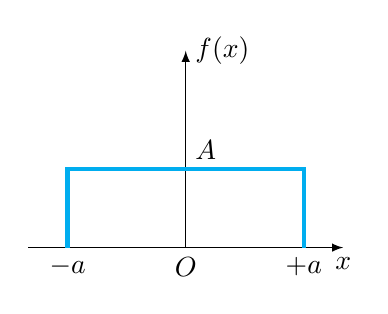
\begin{tikzpicture}
            \label{x的概率密度函数a}
            \draw[-latex] (-2, 0) -- (2, 0) node[below] {$x$};
            \draw[-latex] (0, 0) -- (0, 2.5) node[right] {$f(x)$};
            \node[below] (O) at (0,0) {$O$};

            \draw[ultra thick, cyan] (-1.5, 0) -- (-1.5, 1) -- (1.5, 1) -- (1.5, 0);

            \node[below] at (-1.5, 0) {$-a$};
            \node[below] at (1.5, 0) {$+a$};
            \node[above right] (A) at (0, 1) {$A$};
        \end{tikzpicture}
        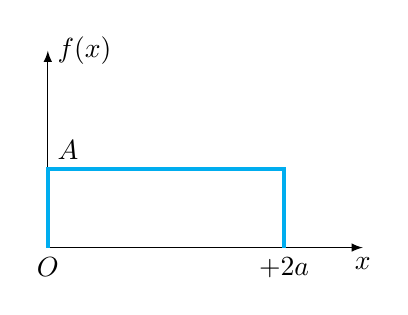
\begin{tikzpicture}
            \label{x的概率密度函数b}
            \draw[-latex] (0, 0) -- (4, 0) node[below] {$x$};
            \draw[-latex] (0, 0) -- (0, 2.5) node[right] {$f(x)$};
            \node[below] at (0,0) {$O$};

            \draw[ultra thick, cyan] (0, 0) -- (0, 1) -- (3, 1) -- (3, 0);

            \node[below] at (3, 0) {$+2a$};
            \node[above right] at (0, 1) {$A$};
        \end{tikzpicture}
        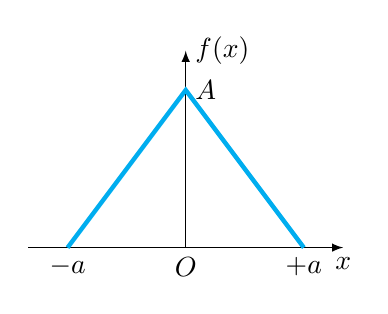
\begin{tikzpicture}
            \label{x的概率密度函数c}
            \draw[-latex] (-2,0) -- (2,0) node[below] {$x$};
            \draw[-latex] (0,0) -- (0,2.5) node[right] {$f(x)$};
            \node[below] at (0,0) {$O$};

            \draw[ultra thick, cyan] (-1.5, 0) -- (0, 2) -- (1.5, 0);

            \node[below] at (-1.5, 0) {$-a$};
            \node[below] at (1.5, 0) {$+a$};
            \node[right] at (0, 2) {$A$};
        \end{tikzpicture}
    \end{center}
\end{question}

\begin{solution}
    连续型随机变量的概率密度有如下性质:
    \begin{equation}
        \int_{-\infty}^{+\infty} f(x) \,\mathrm{d}x = 1
    \end{equation}
    \begin{equation}
        \overline{g(x)} = \int_{-\infty}^{+\infty} f(x)g(x) \,\mathrm{d}x
    \end{equation}

    \paragraph{对于(a)图} 按照归一化条件, 概率密度分布曲线下的面积为 $1$ ,则
    $$
        A = \frac{1}{2a}.
    $$
    $x$ 的概率密度为
    $$
        f(x) = \begin{dcases}
            \frac{1}{2a}, & -a \leqslant x \leqslant a, \\
            0,            & \text{其他}.
        \end{dcases}
    $$
    由此计算 $\overline{x}$ , $\overline{x^2}$ 和 $\overline{|x|}$
    $$
        \overline{x}
        = \int_{-a}^{+a} x f(x) \,\mathrm{d}x
        = \frac{1}{2a}\int_{-a}^{+a} x \,\mathrm{d}x
        = \frac{1}{2a}\left.\frac{x^2}{2}\right|_{-a}^{+a}
        = 0
    $$
    $$
        \overline{x^2}
        = \int_{-a}^{+a} x^2 f(x) \,\mathrm{d}x
        = \frac{1}{2a}\int_{-a}^{+a} x^2 \mathrm{d}x
        = \frac{1}{2a}\left.\frac{1}{3}x^3\right|_{-a}^{+a}
        = \frac{a^2}{3}
    $$
    $$
        \overline{|x|}
        = \int_{-a}^{0} -x f(x) \,\mathrm{d}x + \int_{0}^{a} x f(x) \,\mathrm{d}x
        = \int_{-a}^0 -\frac{1}{2a}x\,\mathrm{d}x + \int_0^a \frac{1}{2a}x\,\mathrm{d}x
        = \frac{a}{2}
    $$

    \paragraph{对于(b)图} 按照归一化条件,概率密度分布曲线下的面积为 $1$ ,则
    $$
        A = \frac{1}{2a}
    $$
    $x$ 的概率密度为
    $$
        f(x) = \begin{dcases}
            \frac{1}{2a}, & 0 \leqslant x \leqslant 2a, \\
            0,            & \text{其他}.                  \\
        \end{dcases}
    $$
    由此计算 $\overline{x}$ 和 $\overline{x^2}$
    $$
        \overline{x}
        = \int_{0}^{2a} x f(x) \,\mathrm{d}x
        = \frac{1}{2a}\int_{0}^{2a} x \,\mathrm{d}x
        = \left.\frac{1}{2a} \frac{x^2}{2}\right|_{0}^{2a}
        = a
    $$
    $$
        \overline{x^2}
        = \int_{0}^{2a} x^2 f(x) \,\mathrm{d}x
        = \frac{1}{2a}\int_{0}^{2a} x^2 \mathrm{d}x
        = \frac{1}{2a} \left.\frac{x^3}{3}\right|_{0}^{2a}
        = \frac{4a^2}{3}
    $$

    \paragraph{对于(c)图} 按照归一化条件,概率密度分布曲线下的面积为 $1$,则
    $$
        A = \frac{1}{a}.
    $$
    $x$ 的概率密度为
    $$
        f(x) = \begin{dcases}
            \frac{1}{a^2}x + \frac{1}{a},  & -a \leqslant x < 0, \\
            -\frac{1}{a^2}x + \frac{1}{a}, & 0 < x \leqslant a,  \\
            0,                             & \text{其他}.          \\
        \end{dcases}
    $$
    由此计算 $\overline{x}$ 和 $\overline{x^2}$
    $$
        \overline{x}
        = \int_{-a}^{+a} x f(x) \,\mathrm{d}x
        = \int_{-a}^{0} \left(\frac{1}{a^2}x^2 + \frac{1}{a}x\right) \mathrm{d}x +  \int_{0}^{a} \left(-\frac{1}{a^2}x^2 + \frac{1}{a}x\right) \mathrm{d}x
        = 0
    $$
    $$
        \overline{x^2}
        = \int_{-a}^{+a} x^2 f(x) \,\mathrm{d}x
        = 2\int_0^a \left(-\frac{1}{a^2}x^3 + \frac{1}{a}x^2 \right) \mathrm{d}x
        =  2\left.\left(-\frac{1}{4a^2}x^4 + \frac{1}{3a}x^3 \right)\right|_0^a = \frac{a^2}{6}
    $$
\end{solution}

\begin{question}{题目2.3.2}
    求速率在区间 $v_p \to 1.01v_p$ 内的气体分子数占总分子数的比率.
\end{question}
\begin{solution}
    麦克斯韦速率分布为
    \begin{equation}
        \frac{\mathrm{d}N}{N} = f(v) \,\mathrm{d}v = 4\pi\left(\frac{m}{2\pi kT}\right)^{3/2} \cdot \exp\left(-\frac{mv^2}{2kT}\right) \cdot v^2 \, \mathrm{d}v
    \end{equation}
    考虑到题目设定的速率区间与 $v_p$ 有关,故考虑用 $v_p = \sqrt{\dfrac{2kT}{m}}$ 改写上式
    $$
        \frac{\mathrm{d}N}{N} = f(v) \,\mathrm{d}v
        = \frac{4}{\sqrt{\pi}}\left(\frac{1}{v_p^2}\right)^{3/2} \cdot \exp\left(-\frac{v^2}{v_p^2}\right) \cdot v^2 \,\mathrm{d}v
    $$
    虽然因式 $\exp\left(-\dfrac{v^2}{v_p^2}\right)$ 很难直接处理,但是我们可以考虑用 $u = \dfrac{v}{v_p}$ 换元,进一步得到
    $$
        \frac{\mathrm{d}N_u}{N} = \frac{4}{\sqrt{\pi}}\left(\frac{1}{v_p^2}\right)^{3/2} \cdot \exp(-u^2) \cdot (uv_p)^2 \,\mathrm{d}(uv_p)  = \frac{4}{\sqrt{\pi}}\cdot\exp(-u^2)\cdot u^2 \,\mathrm{d}u
    $$
    相应地, 速率区间 $v_p \leqslant v \leqslant 1.01v_p$ 也会随着换元而变为 $1 \leqslant u \leqslant 1.01$. 注意到这是一个非常非常窄的区间,所以可以近似认为 $u = 1$, $\mathrm{d}u = 0.01$
    $$
        \frac{\mathrm{d}N_u}{N}
        \approx \frac{4}{\sqrt{\pi}} \cdot \mathrm{e}^{-1} \cdot 1^2 \cdot 0.01
        \approx 0.83\%.
    $$
\end{solution}

\begin{question}{题目2.3.4}
    根据麦克斯韦速率分布,求速率倒数的平均值 $\overline{\left(\dfrac{1}{v}\right)}$
\end{question}

\begin{solution}
    $$
        \begin{aligned}
            \overline{\left(\dfrac{1}{v}\right)}
             & = \int_0^{+\infty} \frac{1}{v} \cdot 4\pi \left(\frac{m}{2\pi kT}\right)^{3/2} \cdot \exp\left(-\frac{mv^2}{2kT}\right) \cdot v^2 \,\mathrm{d}v \\
             & = \int_0^{+\infty} \frac{4}{\sqrt{\pi}}\left(\frac{m}{2kT}\right)^{3/2} \cdot \exp\left(-\frac{mv^2}{2kT}\right) \cdot v \,\mathrm{d}v          \\
        \end{aligned}
    $$
    令 $\alpha = \dfrac{m}{2kT}>0$,$v\mathrm{d}v = \dfrac{1}{2}\mathrm{d}v^2$上式化为
    $$
        \begin{aligned}
            \overline{\left(\dfrac{1}{v}\right)}
             & = \int_0^{+\infty} \frac{4}{\sqrt{\pi}} \alpha^{3/2}  \cdot \exp(-\alpha v^2) \, \frac{1}{2}\mathrm{d}v^2                                      \\
             & = \frac{2}{\sqrt{\pi}}\alpha^{3/2} \int_0^{+\infty} \exp(-\alpha v^2) \,\mathrm{d}v^2                                                          \\
             & = \frac{2}{\sqrt{\pi}}\alpha^{3/2} \cdot \left.\left[\left(-\frac{1}{\alpha}\right) \cdot \mathrm{e}^{-\alpha v^2}\right]\right|_{0}^{+\infty} \\
             & = -\frac{2}{\sqrt{\pi}}\alpha^{1/2} \cdot (\mathrm{e}^{-\infty}-\mathrm{e}^0)                                                                  \\
             & = \sqrt{\frac{2m}{\pi kT}}
        \end{aligned}
    $$
    根据平均速率表达式 $\bar{v} = \sqrt{\dfrac{8kT}{\pi m}}$ ,有
    $$
        \overline{\left(\dfrac{1}{v}\right)} = \frac{4}{\pi} \cdot \frac{1}{\bar{v}}
    $$
\end{solution}

\begin{question}{题目2.3.6}试将麦克斯韦速率分布化为按平动动能的分布,并求出最概然动能.它是否等于 $\dfrac{mv_p^2}{2}$?为什么?
\end{question}

\begin{solution}
    根据平动动能表达式
    $$
        \varepsilon = \frac{1}{2}mv^2
    $$
    解出
    $$
        v = \sqrt{\dfrac{2\varepsilon}{m}}
    $$
    将$f(v) \,\mathrm{d}v$ 改写为 $F(\varepsilon) \,\mathrm{d}\varepsilon$
    $$
        \begin{aligned}
            F(\varepsilon)\,\mathrm{d}\varepsilon
             & = 4\pi\left(\frac{m}{2\pi kT}\right)^{3/2} \cdot \exp\left(-\frac{m}{2kT} \cdot \frac{2\varepsilon}{m}\right) \cdot \frac{2\varepsilon}{m} \,\mathrm{d}\left(\sqrt{\frac{2\varepsilon}{m}}\right)      \\
             & = 4\pi\left(\frac{m}{2\pi kT}\right)^{3/2} \exp\left(-\frac{\varepsilon}{kT}\right) \cdot \frac{2\varepsilon}{m} \cdot \sqrt{\frac{2}{m}} \cdot \frac{1}{2 \sqrt{\varepsilon}} \,\mathrm{d}\varepsilon \\
             & = 2\pi\left(\frac{1}{kT} \right)^{3/2} \exp\left(-\frac{\varepsilon}{kT}\right) \sqrt{\varepsilon} \,\mathrm{d}\varepsilon                                                                             \\
        \end{aligned}
    $$
    再将 $F(\varepsilon)$ 对 $\varepsilon$ 求导,并令导函数为零
    $$
        \left. \frac{\mathrm{d}F(\varepsilon)}{\mathrm{d}\varepsilon} \right|_{\varepsilon=\varepsilon_p} = 0
    $$
    $$
        \frac{2}{\sqrt{\pi}}\left(\frac{1}{kT} \right)^{3/2} \left[ -\frac{1}{kT}\exp\left(-\frac{\varepsilon}{kT}\right) \sqrt{\varepsilon} + \exp\left(-\frac{\varepsilon}{kT}\right)\frac{1}{2\sqrt{\varepsilon}} \right] = 0 \\
    $$
    $$
        \frac{2}{\sqrt{\pi}}\left( \frac{1}{kT} \right)^{3/2} \exp\left(-\frac{\varepsilon}{kT}\right) \left( -\frac{1}{kT}\sqrt{\varepsilon} + \frac{1}{2\sqrt{\varepsilon}} \right) = 0\\
    $$
    前两个因式绝对不为零,当且仅当第三个因式为零时,导函数为零,即
    $$
        -\frac{1}{kT}\sqrt{\varepsilon} + \frac{1}{2\sqrt{\varepsilon}} = 0
    $$
    此时最概然动能 $v_p$ 为
    $$
        \varepsilon_p = \frac{kT}{2}
    $$
    而最概然速率下的动能 $\varepsilon_{v_p}$ 表示为
    $$
        \varepsilon_{v_p}
        = \frac{1}{2}mv_p^2
        = \frac{1}{2}m\left(\frac{2kT}{m}\right)
        = kT
    $$
    可见, 最概然动能 $\varepsilon_p$ 和最概然速率下的动能 $\varepsilon_{v_p}$ 不相等.
\end{solution}

\begin{question}{题目2.4.2}
    分子质量为 $m$ 的气体在温度 $T$ 下处于平衡. 若以 $v_x$ 、$v_y$ 、 $v_z$ 以及 $v$ 分别表示分子速度的$x$、$y$、$z$三个分量及其速率,试求下述平均值:
    \begin{enumerate}
        \item[(1)] $\overline{v_x}$
        \item[(2)] $\overline{v_x^2}$
        \item[(3)] $\overline{v_xv^2}$
        \item[(4)] $\overline{v_x^2v_y}$
        \item[(5)] $\overline{(v_x+bv_y)^2}$
    \end{enumerate}
\end{question}
\begin{solution}
    麦克斯韦速度分布可以表示为
    \begin{equation}
        f(v_i) \,\mathrm{d}v_i = \left(\frac{m}{2\pi kT}\right)^{1/2} \cdot \exp\left(- \frac{mv_i^2}{2kT}\right) \mathrm{d}v_i
        \quad
        (i = x, y, z)
    \end{equation}
    任意分量的平均值 $\overline{v_i}$ 表示为
    \begin{equation}
        \begin{aligned}
            \overline{v_i}
             & = \int_{-\infty}^{+\infty} v_if(v_i) \,\mathrm{d}v_i                                                                    \\
             & =\int_{-\infty}^{+\infty} \left(\frac{m}{2\pi kT}\right)^{1/2} \exp\left(-\frac{mv_i^2}{2kT}\right) v_i \,\mathrm{d}v_i \\
             & =\left(\frac{m}{2\pi kT}\right)^{1/2} \int_{-\infty}^{+\infty} \exp\left(-\frac{mv_i^2}{2kT}\right) v_i \,\mathrm{d}v_i \\
        \end{aligned}
    \end{equation}
    考虑到奇函数 $\displaystyle \exp\left(-\frac{mv_i^2}{2kT} \right) v_i$ 在对称区间 $(-\infty, +\infty)$ 上的积分为零,所以
    \begin{equation}\label{麦克斯韦速度分布的平均值}
        \overline{v_i} = 0
    \end{equation}
    任意分量的平方平均值 $\overline{v_i^2}$ 表示为
    \begin{equation}
        \begin{aligned}
            \overline{v_i^2}
             & = \int_{-\infty}^{+\infty} v_i^2 f(v_i) \,\mathrm{d}v_i                                                                    \\
             & = \int_{-\infty}^{+\infty} \left(\frac{m}{2\pi kT}\right)^{1/2} \exp\left(-\frac{mv_i^2}{2kT}\right) v_i^2 \,\mathrm{d}v_i \\
             & = \left(\frac{m}{2\pi kT}\right)^{1/2} \int_{-\infty}^{+\infty} \exp\left(-\frac{mv_i^2}{2kT}\right) v_i^2 \,\mathrm{d}v_i
        \end{aligned}
    \end{equation}
    考虑到 $\displaystyle \exp\left(-\frac{mv_i^2}{2kT}\right) v_i^2 \,\mathrm{d}v_i$ 是偶函数
    \begin{equation}
        \overline{v_i^2} = 2 \int_{0}^{+\infty}\exp\left(-\frac{mv_i^2}{2kT}\right) v_i^2 \,\mathrm{d}v_i
    \end{equation}
    根据课本 P95 附录 2.1 中的积分公式,可知上式属于 $I(2)$ 类型
    \begin{equation}
        \label{麦克斯韦速度分布的方均值}
        \overline{v_i^2}
        = \left(\frac{m}{2\pi kT}\right)^{1/2} \cdot 2 \cdot \frac{1}{4} \sqrt{\pi} \left(\frac{m}{2kT}\right)^{-3/2}
        =\frac{kT}{m}
    \end{equation}
    %\end{tcolorbox}
    (1) 根据公式 $\eqref{麦克斯韦速度分布的平均值}$, 当 $i = x$ 时,有
    $$
        \overline{v_x} = 0
    $$
    (2) 根据公式 $\eqref{麦克斯韦速度分布的方均值}$,当 $i = x$ 时,有
    $$
        \overline{v_x^2} =\frac{kT}{m}
    $$
    (3) 由于 $v_x$ 与 $v$ 相互独立,根据公式 $\eqref{麦克斯韦速度分布的平均值}$
    $$
        \overline{v_x v^2} = \overline{v_x} \cdot \overline{v^2} = 0 \cdot \frac{3kT}{m} = 0
    $$
    (4) 由于 $v_x$ 与 $v$ 相互独立,根据公式 $\eqref{麦克斯韦速度分布的平均值}$
    $$
        \overline{v_x^2 v_y} = \overline{v_x^2} \cdot \overline{v_y} = \frac{kT}{m} \cdot 0 = 0
    $$
    (5) 由于 $v_x$ 与 $v_y$ 相互独立,根据公式 $\eqref{麦克斯韦速度分布的方均值}$ 和 $\eqref{麦克斯韦速度分布的平均值}$
    $$
        \begin{aligned}
            \overline{(v_x + bv_y)^2}
             & = \overline{v_x^2 + 2bv_xv_y + b^2v_y^2}                                                       \\
             & = \overline{v_x^2} + \overline{2bv_xv_y} + \overline{b^2v_y^2}                                 \\
             & = \overline{v_x^2} + 2b \cdot \overline{v_x} \cdot \overline{v_y} + b^2 \cdot \overline{v_y^2} \\
             & = \frac{kT}{m} + 0 + b^2 \cdot \frac{kT}{m}                                                    \\
             & = \frac{kT}{m}(1+b^2)
        \end{aligned}
    $$
\end{solution}

\begin{question}{题目2.4.5}
    求麦克斯韦速度分布中速度分量 $v_x > 2v_p$ 的分子数占总分子数的比率.
\end{question}
\begin{solution}
    根据麦克斯韦速度分布,有
    $$
        \frac{\mathrm{d}N(v_x)}{N}
        = \int_{2v_p}^{+\infty} \left(\frac{m}{2 \pi kT}\right)^{1/2} \cdot \exp\left(-\frac{mv_x^2}{2kT}\right) \,\mathrm{d}v_x
    $$
    令 $u =  \dfrac{v_x}{v_p}$
    $$
        \frac{\mathrm{d}N}{N}
        = \left(\frac{m}{2 \pi kT}\right)^{1/2} \int_{2}^{+\infty} \exp(-u^2) \,\mathrm{d}(u \cdot v_p)
        = \frac{1}{\sqrt{\pi}}\int_{2}^{+\infty} \exp(-u^2) \,\mathrm{d}u
    $$
    我们在此处引入误差函数 $\displaystyle \operatorname{erf}(x) = \dfrac{2}{\sqrt{\pi}}\int_0^x \exp(-x^2) \,\mathrm{d}x$,上式化为
    $$
        \begin{aligned}
            \frac{\mathrm{d}N}{N}
             & = \frac{1}{2} \left[ \frac{2}{\sqrt{\pi}}\int_{2}^{+\infty} \exp(-u^2) \,\mathrm{d}u \right] \\
             & = \frac{1}{2} \left[\frac{2}{\sqrt{\pi}}\int_0^{+\infty}\exp(-u^2) \,\mathrm{d}u
            - \frac{2}{\sqrt{\pi}}\int_0^2\exp(-u^2) \,\mathrm{d}u  \right]                                 \\
             & = \frac{1}{2} \left[ 1- \operatorname{erf} (2)\right]                                        \\
             & \approx 0.00235
        \end{aligned}
    $$
    % \begin{center}
    %     \begin{tikzpicture}[scale = 2]
    %         \draw[smooth, domain = -2 : 2] plot(\x, exp{-\x*\x});
    %         \draw[-latex] (-2.5, 0) -- (2.5, 0) node[below] {$x$};
    %         \draw[-latex] (0, 0) -- (0, 1.5) node[left] {$y$};
    %         \node[below] at (0, 0) {$O$};
    %         \draw[cyan] (-2, 1) -- (2, 1);
    %     \end{tikzpicture}
    % \end{center}
    综上所述,麦克斯韦速度分布中速度分量 $v_x > 2v_p$ 的分子数占总分子数的比率为 $0.235\%$.
\end{solution}

\begin{question}{题目2.5.2}
    一容器被一隔板分成两部分,其中气体的压强分别为 $p_1$ 和 $p_2$.两部分气体的温度均为 $T$,摩尔质量均为 $M$.试证明:如果隔板上有一面积为 $A$ 的小孔,则每秒通过小孔的气体质量为
    $$
        \frac{\mathrm{d}m}{\mathrm{d}t} = \sqrt{\frac{M}{2\pi RT}} |p_1 - p_2| A.
    $$
\end{question}

\begin{solution}
    根据平均速率公式 $\bar{v}$ 和压强公式 $p$ ,可以把气体分子碰撞公式 $\Gamma$ 变换为
    $$
        \begin{dcases}
            \bar{v} = \sqrt{\frac{8kT}{\pi m}} \\
            p=\frac{1}{3}nm\overline{v^2}      \\
            \Gamma = \frac{1}{4} n \bar{v}
        \end{dcases}
        \implies \Gamma = \frac{p}{\sqrt{2\pi mkT}}
    $$
    我们不妨用下标 $1$ 和 $2$ 分别表示隔板左右的各个物理量,那么单位时间内通过单位面积小孔的分子数应表示为
    $$
        \Delta \Gamma = |p_1 - p_2| \cdot \frac{1}{\sqrt{2\pi mkT}}
    $$
    由此可知在 $\mathrm{d}t$ 时间内通过小孔的气体质量为
    $$
        \mathrm{d}m = m \cdot \Delta\Gamma \cdot A \cdot \mathrm{d}t
    $$
    每秒通过小孔的气体质量可以表示为
    $$
        \frac{\mathrm{d}m}{\mathrm{d}t} = \sqrt{\frac{m}{2\pi kT}} \cdot|p_1-p_2| \cdot A = \sqrt{\frac{M}{2\pi RT}} |p_1 - p_2| A.
    $$
\end{solution}

\begin{question}{题目2.5.8}
    一带有小孔(小孔面积为 $A$ )的固定隔板把容器分为体积均为 $V$ 的两部分. 开始时,左方装有温度为 $T_0$、压强为 $p_0$ 的单原子分子理想气体,右方为真空. 由于孔很小,因而虽然板两边分子数随时间变化,但仍可假定任一时刻近似是平衡态,又整个容器被温度为$T_0$ 的热源包围. 试求:
    \begin{enumerate}
        \item[(1)] 在 $t \to t+\mathrm{d}t$ 时间内从左方穿过小孔到达右方的分子;
        \item[(2)] 左方压强的具体表达式(它是时间的函数);
        \item[(3)] 最后达到平衡时气体与热源一共交换了多少热量?
    \end{enumerate}
\end{question}

\begin{solution}
    (1)左方和右方容器都有分子穿过小孔到达对方容器. 设 $t$ 时刻左方和右方容器中的分子数密度分别为 $n_1(t)$,$n_2(t)$,由于左右两个容器的体积相等,并且初始时刻右方容器压强为零,所以
    $$
        n_1(t) + n_2(t) = n_0 \left( \text{其中} n_0 = \frac{p_0}{kT} \right)
    $$
    按照气体分子的碰撞数公式,在 $t \to t+\mathrm{d}t$ 时间内从左侧穿越小孔到达右侧的分子数为
    $$
        -\mathrm{d}N_1 = \frac{n_1\bar{v}A\mathrm{d}t}{4} - \frac{n_2\bar{v}A\mathrm{d}t}{4}
    $$
    (2)联立以上两式,可得
    $$
        \mathrm{d}n_1 = -\frac{A\bar{v}}{4V} \cdot \left(2n_1 - n_0\right) \mathrm{d}t
    $$
    两边同除以 $V$ 得到左右两侧的压强关系,其中 $p_1$ 是关于时间 $t$ 的函数
    $$
        \mathrm{d} p_1  = -\frac{A\bar{v}}{4V} \cdot (2p_1 - p_0) \mathrm{d}t
    $$
    分离变量并积分
    $$
        \begin{aligned}
            \mathrm{d}p_1                                          & = -\frac{A\bar{v}}{4V} \cdot (2p_1 - p_0) \mathrm{d}t \\
            \frac{\mathrm{d}p_1}{2p_1 - p_0}                       & =  -\frac{A\bar{v}}{4V} \mathrm{d}t                   \\
            \int_{p_0}^{p_1} \frac{\mathrm{d}p_1}{2p_1 - p_0}      & = \int_0^t -\frac{A\bar{v}}{4V} \mathrm{d}t           \\
            \left. \frac{1}{2} \ln(2p_1 - p_0) \right|_{p_0}^{p_1} & = \left. -\frac{A\bar{v}}{4V} t \right|_0^t           \\
            \ln(2p_1 - p_0)                                        & = -\frac{A\bar{v}}{2V} t + \ln{p_0}                   \\
        \end{aligned}
    $$
    把等式两边同时作为 $\mathrm{e}$ 的指数,并化简得
    $$
        p_1(t) = \frac{p_0}{2} \cdot \left[1+\exp\left(-\frac{A\bar{v}}{4V}t\right) \right]
    $$
    (3)由于两边的容器温度始终为 $T_0$, 且系统和外面的温度始终相等,所以最后达到平衡的过程中气体与热源之间没有热量交换.
\end{solution}

\begin{question}{题目2.7.1}
    求常温下质量 $m_1=3.00 \,\si{g}$ 的水蒸气与 $m_2 = 3.00 \,\si{g}$ 的氢气组成的混合理想气体的摩尔定容热容.
\end{question}

\begin{solution}
    考虑到$m_1=3.00 \,\si{g}$ 的水蒸气的物质的量为 $\dfrac{1}{6} \,\si{mol}$,有$6$个自由度;$m_2 = 3.00 \,\si{g}$ 的氢气的物质的量为 $\dfrac{3}{2} \,\si{mol}$,有$5$个自由度,所以气体的内能可以表示为
    $$
        U = \frac{1}{6} \cdot \frac{6}{2}RT + \frac{3}{2} \cdot \frac{5}{2}RT
        = \frac{17}{4}RT
    $$
    所以 $1 \,\si{mol}$ 此种理想气体所具有的内能 $U_\mathrm{m}$可以表示为
    $$
        U_\mathrm{m} = \frac{U}{\frac{1}{6} + \frac{3}{2}} = \frac{51}{20}RT
    $$
    而此气体的摩尔定容热容可以表示为
    $$
        C_{V,\mathrm{m}}
        = \frac{\mathrm{d}U_\mathrm{m}}{\mathrm{d}T}
        = 21.2 \,\si{J \cdot mol^{-1} \cdot K^{-1}}
    $$
\end{solution}

\begin{question}{题目2.7.2}
    某种气体分子由四个原子组成,它们分别处在四面体的四个顶点上
    \begin{enumerate}
        \item[(1)] 求这种分子的平动自由度数、转动自由度数和振动自由度数;
        \item[(2)] 根据能量均分定理求这种气体的摩尔定容热容
    \end{enumerate}
\end{question}

\begin{solution}
    \begin{itemize}
        \item[(1)] 这种气体分子有 $3$ 个平动自由度,$3$个转动自由度,振动自由度数最多可以有 $6$ 个;
        \item[(2)] 如果为刚性分子,其振动自由度全部被冻结,这时有 $3$ 个平动自由度和 $3$ 个转动自由度。按照能量均分定理,摩尔定容热容为 $C_{V,\mathrm{m}} = 6 \cdot \frac{R}{2} = 3R$.
    \end{itemize}
\end{solution}
\section{热力学第一定律}
\begin{question}{题目4.2.1}
    $1 \,\si{mol}$ 气体做准静态等温膨胀,由初体积$V_\mathrm{i,m}$ 变成终体积 $V_\mathrm{f,m}$,试计算这过程中系统对外界所做的功. 物态方程分别为
    \begin{enumerate}
        \item[(1)] $p(V_\mathrm{m} - b) = RT$ ($R$,$b$是常量)
        \item[(2)] $pV_\mathrm{m} = RT\left(1-\dfrac{B}{V_\mathrm{m}}\right)$ ($R$为常量,$B = f(T)$)
    \end{enumerate}
\end{question}

\begin{solution}
    (1)根据题目所给的物态方程,得到压强 $p$ 的表达式为
    $$
        p = \frac{RT}{V_\mathrm{m} - b}
    $$
    准静态等温膨胀过程中所做的功为
    $$
        W  = \int_{V_\mathrm{i,m}}^{V_\mathrm{f,m}} p \,\mathrm{d}V_\mathrm{m}
        = \int_{V_\mathrm{i,m}}^{V_\mathrm{f,m}} \frac{RT}{V_\mathrm{m} - b} \,\mathrm{d}V_\mathrm{m}
        = RT\ln\frac{V_\mathrm{f,m} - b}{V_\mathrm{i,m} - b}
    $$
    (2)根据题目所给的物态方程,得到压强 $p$ 的表达式为
    $$
        p = RT\left(\frac{1}{V_\mathrm{m}} - \frac{B}{V_\mathrm{m}^2}\right)
    $$
    准静态等温膨胀过程中所做的功为
    $$
        W  = \int_{V_\mathrm{i,m}}^{V_\mathrm{f,m}} p \,\mathrm{d}V_\mathrm{m}
        = RT \int_{V_\mathrm{i,m}}^{V_\mathrm{f,m}} \left(\frac{1}{V_\mathrm{m}} - \frac{B}{V_\mathrm{m}^2} \right) \,\mathrm{d}V_\mathrm{m}
        = RT\ln\frac{V_\mathrm{f,m}}{V_\mathrm{i,m}} + \frac{BRT}{V_\mathrm{f,m}} - \frac{BRT}{V_\mathrm{i,m}}
    $$
\end{solution}

\begin{question}{题目4.4.2}
    已知范德瓦耳斯气体物态方程为
    $$
        \left(p+\frac{a}{V_\mathrm{m}^2}\right)\left(V_\mathrm{m}-b\right) = RT,
    $$
    其内能为
    $$
        U_\mathrm{m} = cT - \frac{a}{V_\mathrm{m}^2} + d,
    $$
    其中 $a$,$b$,$c$,$d$ 均为常量.试求:
    \begin{enumerate}
        \item[(1)] 该气体从 $V_1$ 等温膨胀到 $V_2$ 时系统对外界所做的功;
        \item[(2)] 该气体在定体下升高 $\Delta T$ 温度所吸收的热量.
    \end{enumerate}
\end{question}
\begin{solution}
    (1)改写方程得到 $p$ 的表达式,并代入做功表达式
    $$
        W'  = \int_{V_\mathrm{1,m}}^{V_\mathrm{2,m}} p \,\mathrm{d}V_\mathrm{m}
        = \int_{V_\mathrm{1,m}}^{V_\mathrm{2,m}} \left(\frac{RT}{V_\mathrm{m}-b} - \frac{a}{V_\mathrm{m}^2} \right) \,\mathrm{d}V_\mathrm{m}
        = RT\ln\frac{V_\mathrm{2,m} - b}{V_\mathrm{1,m}-b} + \frac{a}{V_\mathrm{2,m}} - \frac{a}{V_\mathrm{1,m}}.
    $$
    (2)定体情况下气体不向外做功,所以吸收的热量会全部转化为气体内能
    $$
        \Delta{Q} = \Delta{U} = c( T + \Delta T ) - \frac{a}{V_\mathrm{m}^2} + d -\left(cT - \frac{a}{V_\mathrm{m}^2} + d\right) = c \cdot \Delta{T}.
    $$
\end{solution}

\begin{question}{题目4.4.4}
    实验数据表明,在 $0.1 \,\si{MPa}$,$300-1200 \,\si{K}$ 范围内铜的摩尔定压热容为 $C_{p,\mathrm{m}} = a + bT$,其中 $a = 2.3 \times 10^{4} \,\si{J \cdot mol^{-1} \cdot K^{-1}}$,$b = 5.92 \,\si{J \cdot mol^{-1} \cdot K}$. 试计算在 $0.1 \,\si{MPa}$ 下,温度从 $300\,\si{K}$ 增到 $1200\,\si{K}$ 时铜的摩尔焓的改变.
\end{question}
\begin{solution}
    由于温度在 $300 \,\si{K}$ 增到 $1200\,\si{K}$ 的过程中铜的压强不变,因而它吸收的热量等于焓的改变
    $$
        H_\mathrm{m} = \Delta{Q}_\mathrm{m} = \int_{T_1}^{T_2} C_{p,\mathrm{m}} \,\mathrm{d}T = \int_{T_1}^{T_2} (a+bT) \,\mathrm{d}T = 2.47 \times 10^7 \,\si{ J \cdot mol^{-1} }
    $$
\end{solution}

\begin{question}{题目4.4.6}
    设 $1 \,\si{mol}$ 固体的物态方程可写为
    $$
        V_\mathrm{m} = V_\mathrm{0,m} + aT + bp,
    $$
    摩尔内能可表示为
    $$
        U_\mathrm{m} = cT - apT,
    $$
    其中 $a,b,c,V_\mathrm{0,m}$均是常量,试求:
    \begin{enumerate}
        \item[(1)] 摩尔焓的表达式
        \item[(2)] 摩尔热容 $C_{p,\mathrm{m}}$ 和 $C_{V,\mathrm{m}}$
    \end{enumerate}
\end{question}
\begin{solution}
    (1)根据焓的定义 $H = U + pV$ 我们有
    $$
        H_\mathrm{m} = U_\mathrm{m} + pV_\mathrm{m} = cT + pV_{0,\mathrm{m}} + bp^2.
    $$
    (2)根据摩尔热容的定义 $C_{p,\mathrm{m}} = \left( \dfrac{\partial H_\mathrm{m}}{\partial T}\right)_p$ 我们有
    $$
        C_{p,\mathrm{m}} = \left( \frac{\partial H_\mathrm{m}}{\partial T}\right)_p = c
    $$
    对于 $1 \,\si{mol}$ 固体,有
    $$
        V_\mathrm{m} = V_{0,\mathrm{m}} + aT + bp
        \implies
        p = \frac{V_\mathrm{m} - V_\mathrm{0,m} - aT}{b}
    $$
    则内能可以表示为
    $$
        U_\mathrm{m}
        = cT - apT
        = cT - a\frac{V_\mathrm{m} - V_\mathrm{0,m} - aT}{b}T
    $$
    于是根据摩尔热容的定义 $C_{V,\mathrm{m}} = \left( \dfrac{\partial U_\mathrm{m}}{\partial T}\right)_V$ 我们有
    $$
        C_{V,\mathrm{m}}
        = \left(\frac{\partial U_\mathrm{m}}{\partial T}\right)_V
        = c - \frac{a}{b}V_\mathrm{m} + \frac{aV_{0,\mathrm{m}}}{b} + \frac{2a^2T}{b}.
    $$
\end{solution}

\begin{question}{题目4.5.1}
    有一除底部外都是绝热的气筒,被一位置固定的导热板隔成相等的两部分 $A$ 和 $B$,其中各盛有 $1 \,\si{mol}$ 的理想气体氮. 今将 $334.4\,\si{J}$ 的热量缓慢地由底部供给气体,设活塞上的压强始终保持为 $0. 101 \,\si{MPa}$,求 $A$ 部和 $B$ 部温度的改变以及各吸收的热量(导热板的热容可以忽略).若将位置固定的导热板换成可以自由滑动的绝热隔板,重复上述讨论.
\end{question}
\begin{solution}
    (1) $A$部经历等体过程
    $$
        \Delta Q_A = \Delta U_\mathrm{m} = C_{V,\mathrm{m}}\Delta{T_A}
    $$
    $B$部经历等压过程
    $$
        \Delta Q_B = \Delta H_\mathrm{m} = C_{p,\mathrm{m}}\Delta{T_B}
    $$
    由于隔板是导热的,所以稳态时 $T_A = T_B$ ,也即 $\Delta T_A = \Delta T_B = \Delta T$,而体系吸收的总热量为 $\Delta Q = 334.4 \,\si{J}$
    $$
        \Delta Q = \Delta{Q_A} + \Delta{Q_B}
        = (C_{V,\mathrm{m}} +C_{p,\mathrm{m}})\Delta{T}
        = 6R \cdot \Delta{T}
        =  334.4 \,\si{J}
    $$
    进一步解得 $\Delta T$,$\Delta Q_A$ 和 $\Delta Q_B$
    $$
        \Delta T = 6.70 \,\si{K}
    $$
    $$
        \Delta Q_A = C_{V,\mathrm{m}}\Delta{T} = \frac{5}{2}R\Delta{T} = 139.27 \,\si{J}
    $$
    $$
        \Delta Q_B = C_{p,\mathrm{m}}\Delta{T} = \frac{7}{2}R\Delta{T} = 194.97 \,\si{J}
    $$
    (2) 若隔板是可以自由滑动的而且是绝热的,则 $A$ 部吸收热量后按照等压过程变化; $B$ 部不吸收热量,也不做功(因为它通过活塞和外界相连接,它的压强始终和外界相等),按照热力学第一定律,其内能不变,状态也不变. $A$ 部吸收的热量全部用于 $A$ 部内能的增加和它对外做的等压功.
    $$
        \Delta Q_A = C_{p,\mathrm{m}} \Delta{T}
        = \frac{7}{2}R\Delta{T} = 334.4 \,\si{K}
    $$
    $$
        \Delta T = \frac{\Delta Q}{\frac{7}{2}R}
        = 11.49 \,\si{K}.
    $$
    $B$ 部与活塞连接,压强恒为$1 \,\si{atm}$,且因为隔板是隔热的,所以它不吸收热量,也不对外做功.
\end{solution}

\begin{question}{题目4.5.2}
    分别通过下列过程把标准状态下的 $0.14 \,\si{kg}$ 氮气压缩为原体积的一半:
    \begin{enumerate}
        \item[(1)] 等温过程;
        \item[(2)] 绝热过程;
        \item[(3)] 等压过程;
    \end{enumerate}
    试分别求出在这些过程中气体内能的改变,传递的热量和外界对气体所做的功,设氮气可看做理想气体,且 $C_{V,\mathrm{m}} = \dfrac{5}{2}R$.
\end{question}
\begin{solution}
    (1)等温过程中 $\Delta{U} = 0$,外界对气体做的功为
    $$
        W = - \nu RT \ln \frac{V_2}{V_1} = 7862 \,\si{J}
    $$
    气体对外放热
    $$
        \Delta{Q} = 7862 \,\si{J}
    $$
    (2)绝热过程中 $\Delta{Q} = 0$,根据绝热过程方程,有
    $$
        T_2 = \left(\frac{V_1}{V_2}\right)^{\gamma - 1} T_1
    $$
    外界对气体做的功为
    $$
        W  = \Delta{U} = \nu C_{V,\mathrm{m}} (T_2 - T_1)
        = \nu C_{V,\mathrm{m}}T_1\left[ \left(\frac{V_1}{V_2}\right)^{\gamma - 1} -1 \right]
        = 9061 \,\si{J}
    $$
    (3)等压过程有 $\frac{T_2}{V_2} = \frac{T_1}{V_1}$,气体内能的变化为
    $$
        \Delta{U}
        = \nu C_{V,\mathrm{m}} (T_2 - T_1)
        = \nu C_{V,\mathrm{m}} T_1 \left( \frac{V_1}{V_2} - 1 \right)
        = -1.41 \times 10^4 \,\si{J}
    $$
    气体放热为
    $$
        \Delta{Q} = \nu C_{p,\mathrm{m}} (T_2 - T_1) = -1.97 \times 10^4 \,\si{J}
    $$
    外界对气体做功
    $$
        W = \Delta{U} - \Delta{Q} = 5.6 \times 10^3 \,\si{J}
    $$
\end{solution}

\begin{question}{题目4.5.3}
    在标准状态下的 $0.016 \,\si{kg}$ 的氧气,分别经过下列过程从外界吸收了 $334.4 \,\si{J}$ 的热量:
    \begin{enumerate}
        \item[(1)] 若为等温过程,求终态体积;
        \item[(2)] 若为等容过程,求终态压强;
        \item[(3)] 若为等压过程,求气体内能的变化;
    \end{enumerate}
    设氧气可看做理想气体,且 $C_{V, \mathrm{m}} = \dfrac{5}{2}R$
\end{question}
\begin{solution}
    初始状态下氧气的各项参量:
    $$
        \nu = \frac{m}{M} = 0.5 \,\si{mol}
        \quad \quad
        p_1 = 1.01 \times 10^5 \,\si{Pa}
        \quad \quad
        T_1 = 273.15 \,\si{K}
        \quad \quad
        V_1 = 11.2 \,\si{L}
    $$
    (1)气体吸热后等温膨胀,内能不变,吸收的热量全部对外做功
    $$
        Q = W  = \int_{V_1}^{V_2} p_1 \,\mathrm{d}V
        = \int_{V_1}^{V_2} \frac{\nu RT_1}{V} \,\mathrm{d}V
        = \nu RT_1 \ln\frac{V_2}{V_1}
    $$
    解得
    $$
        V_2 = V_1 \exp \left(\frac{Q}{\nu RT_1}\right) = 15.04 \,\si{L}
    $$
    (2)气体吸热后等体升温,根据物态方程 $pV = \nu RT$,有
    $$
        \frac{p_1}{T_1} = \frac{p_2}{T_2}
    $$
    同时,等体过程中气体吸收的热量会全部转化为内能
    $$
        Q = U_\mathrm{m} = \nu C_{V,\mathrm{m}}(T_2 - T_1)
        = \frac{5\nu R}{2} \left(\frac{p_2}{p_1} - 1\right)T_1
        = 334.4 \,\si{J}
    $$
    解得 $p_2$
    $$
        p_2 = \left(\frac{2Q}{5 \nu RT_1}+1 \right) p_1 = 1.13 \times 10^5 \,\si{Pa}
    $$
    (3)气体吸热后等压膨胀,吸热过程可以表示为
    $$
        Q = \nu C_{p,\mathrm{m}} (T_2 -T_1) = 334.4 \,\si{J}
    $$
    而内能变化可以表示为
    $$
        U_\mathrm{m} = \nu C_{V,\mathrm{m}}(T_2 - T_1)
        = \frac{Q}{C_{p,\mathrm{m}}} C_{V,\mathrm{m}}
        = 238.86 \,\si{J}
    $$
\end{solution}

\begin{question}{题目4.5.5}
    室温下一定量理想气体氧的体积为 $2.3 \,\si{L}$,压强为 $0.1 \,\si{MPa}$,经过某一多方过程后体积变为 $4.1 \,\si{L}$,压强为 $0.05 \,\si{MPa}$.设氧气 $C_{V, \mathrm{m}} = \dfrac{5}{2}R$,试求:
    \begin{enumerate}
        \item[(1)] 多方指数 $n$;
        \item[(2)] 内能的变化;
        \item[(3)] 吸收的热量;
        \item[(4)] 氧膨胀时对外界所做的功;
    \end{enumerate}
\end{question}
\begin{solution}
    (1)多方过程的方程为 $pV^n = C$,即
    $$
        p_1V_1^n =p_2V_2^n
    $$
    移项整理并取对数,解得
    $$
        n = \frac{
            \ln \left(\dfrac{p_1}{p_2}\right)
        }{
            \ln \left(\dfrac{V_2}{V_1}\right)
        }
        = 1.20
    $$
    (2)根据物态方程 $pV = \nu RT$可以得到
    $$
        p_1V_1 = \nu RT_1
        \quad \quad
        p_2V_2 = \nu RT_2
    $$
    而理想气体的内能变化可以表示为
    $$
        \Delta U
        = \nu C_{V,\mathrm{m}}(T_2 -T_1)
        = \nu \frac{5R}{2} \left(\frac{p_2V_2}{\nu R} - \frac{p_1V_1}{\nu R}\right)
        = -62.5 \,\si{J}
    $$
    (3)多方过程的热容为
    $$
        C_{n,m} = C_{V,m} - \frac{R}{n-1}
    $$
    多方过程中吸收的热量为
    $$
        Q = \nu C_{n,m} (T_2 - T_1)
        = \nu \left(\frac{5R}{2} - \frac{R}{1.20 - 1}\right) \left(\frac{p_2V_2}{\nu R} - \frac{p_1V_1}{\nu R}\right)
        = 62.5 \,\si{J}
    $$
    (4) 根据热力学第一定律,系统内能变化为
    $$
        \Delta U = Q + W
    $$
    则系统对外做功 $W'$ 可以表示为
    $$
        W' = -W = Q - \Delta{U} = 62.5 - (-62.5) = 125 \,\si{J}
    $$
\end{solution}

\begin{question}{题目4.5.16}
    有 $28 \,\si{g}$ 氮气经摩尔热容 $C_{1,\mathrm{m}} =2R$ 的平衡过程,从标准状态开始体积膨胀了 $4$ 倍. 试问:
    \begin{enumerate}
        \item[(1)] 该过程满足什么样的方程?
        \item[(2)] 在该过程中对外做了多少功,改变了多少内能,吸(或放)了多少热量?
    \end{enumerate}
\end{question}
\begin{solution}
    (1)根据热力学第一定律,可知此过程中氮气吸收的热量会转化为自身内能和对外做功
    $$
        C_{V,\mathrm{m}} \,\mathrm{d}T = C_{1,\mathrm{m}} \,\mathrm{d}T - p \,\mathrm{d}V
    $$
    其中 28g 氮气的 $C_{V,\mathrm{m}} = \dfrac{5R}{2}$,$C_{1,\mathrm{m}} = 2R$, $\nu = 1 \,\si{mol}$
    $$
        \frac{R}{2} \ \mathrm{d}T = -p \ \mathrm{d}V
    $$
    根据物态方程 $pV = \nu RT$ 消去 $T$,并分离变量
    $$
        \begin{aligned}
            \frac{R}{2} \,\mathrm{d}\left(\frac{pV}{R}\right)      & = -p \,\mathrm{d}V         \\
            \frac{1}{2} \left(p\,\mathrm{d}V + V\mathrm{d}p\right) & = -p \,\mathrm{d}V         \\
            \frac{\mathrm{d}p}{p}                                  & = -3 \frac{\mathrm{d}V}{V} \\
        \end{aligned}
    $$
    两边积分并整理
    $$
        \begin{aligned}
            \int\frac{\mathrm{d}p}{p} & = -3 \int\frac{\mathrm{d}V}{V} \\
            \ln{p} + C_1              & = -3\ln{V} + C_2               \\
            pV^3                      & = C
        \end{aligned}
    $$
    \paragraph{方法二}
    根据理想气体多方过程的热容公式,求出 $C_{n,\mathrm{m}}$
    $$
        C_{n,\mathrm{m}}
        = C_{V,\mathrm{m}} - \frac{R}{n-1}
        = C_{V,\mathrm{m}} \cdot \frac{\gamma-n}{1-n}
        = 3
    $$
    于是方程为
    $$
        pV^3 = C
    $$
    (2) $28 \,\si{g}$ 氮气在标准状态下时
    $$
        \nu = 1 \,\si{mol},
        \quad\quad
        p_0 = 1.01 \times 10^5 \,\si{Pa},
        \quad\quad
        V_0 = 22.4 \,\si{L},
        \quad\quad
        T_0 = 273.15\,\si{K}
    $$
    经历多方过程后,体积膨胀为初始状态的 $4$ 倍($V_2 = 4V_0 = 89.6 \,\si{L}$)压强变为 $p_2$
    $$
        p_2 = p_1 \left(\dfrac{V_1}{V_2}\right)^3
        = \frac{12625}{8} \,\si{Pa}
    $$
    温度变为
    $$
        T_2 = \dfrac{p_1V_1}{p_2V_2}T_1 = \frac{5463}{320} \,\si{K}
    $$
    氮气的内能改变量 $\Delta U$ 为
    $$
        \Delta U
        = \nu C_{V,\mathrm{m}} (T_2-T_1)
        %= 1 \times \frac{5R}{2} \times \left(\frac{5463}{320} - 273.15\right)
        = - 5324.63 \,\si{J}
    $$
    氮气吸收的热量 $\Delta Q$ 为
    $$
        \Delta Q
        = \nu  C_{1,\mathrm{m}} (T_2 - T_1)
        %= 1 \times 2R \times \left(\frac{5463}{320} - 273.15\right)
        = -4259.71 \,\si{J}
    $$
    系统对外做功 $W'$ 为
    $$
        W' = -W = \Delta Q - \Delta U =  1064.92 \,\si{J}
    $$
\end{solution}

\begin{question}{题目4.6.1}
    已知某种理想气体在 $p-V$ 图上的等温线与绝热线的斜率之比为 $0.714$,现 $1 \,\si{mol}$ 该种理想气体在 $p-T$ 图上经历如图所示的循环,试问:
    \begin{enumerate}
        \item [(1)] 该气体的 $C_{V,\mathrm{m}}$ 是多少?
        \item [(2)] 循环中所做的功是多少?
        \item [(3)] 循环效率是多少?
    \end{enumerate}
    \centering
    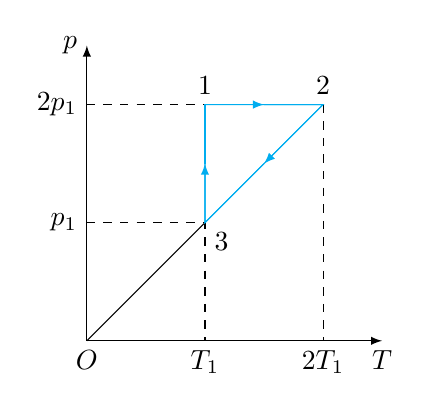
\begin{tikzpicture}[scale = 1.5, domain = 0:3]
        %画坐标轴
        \draw[-latex] (0,1) -- (0, 0) -- (2.5, 0) node[below] {$T$};
        \draw[-latex] (1,0) -- (0, 0) -- (0, 2.5) node[left ] {$p$};
        \node[below] at (0,0) {$O$};

        %画出虚线辅助线
        \draw (0, 0) -- (1, 1);
        \draw[dashed] (0, 1) -- (1, 1) -- (1, 0);
        \draw[dashed] (0, 2) -- (1, 2);
        \draw[dashed] (2, 2) -- (2, 0);

        %画出三个循环的箭头
        \draw[-latex, cyan] (1, 1.5) -- (1,2) -- (1.5, 2);
        \draw[-latex, cyan] (1.5, 2) -- (2,2) -- (1.5, 1.5);
        \draw[-latex, cyan] (1.5, 1.5) -- (1,1) -- (1, 1.5);
        \draw[cyan] (1, 1) -- (1, 2) -- (2, 2) -- (1, 1) -- cycle;

        %标注出各个点
        \node[left] at (0, 1) {$p_1$};
        \node[left] at (0, 2) {$2p_1$};
        \node[below] at (1, 0) {$T_1$};
        \node[below] at (2, 0) {$2T_1$};
        \node[above] at (1, 2) {$1$};
        \node[above] at (2, 2) {$2$};
        \node[below right] at (1, 1) {$3$};
    \end{tikzpicture}
\end{question}

\begin{solution}
    (1)对等温过程方程$pV = \nu RT$两边取微分
    $$
        \partial{(pV)} = \partial{(\nu RT)}
    $$
    $$
        V \partial{p} + p \partial{V} = 0
    $$
    得到等温 $p-V$ 曲线的斜率
    $$
        \left( \frac{\partial p}{\partial V} \right)_T = -\frac{p}{V}
    $$
    对绝热过程方程$pV^{\gamma} = C$两边取微分
    $$
        \partial \left(pV^{\gamma}\right) = \partial(C)
    $$
    $$
        \partial{p} \, V^\gamma + p \, \gamma V^{\gamma - 1} \partial{V} = 0
    $$
    得到绝热 $p-V$ 曲线的斜率
    $$
        \left( \frac{\partial p}{\partial V} \right)_S = -\gamma \frac{p}{V}
    $$
    由于等温线与绝热线的斜率之比为 $0.714$,所以
    $$
        \frac{
            \left(\dfrac{\partial p}{\partial V}\right)_T
        }{
            \left(\dfrac{\partial p}{\partial V}\right)_S
        }
        =\frac{1}{\gamma}
        = \frac{ C_{V,\mathrm{m}} }{ C_{p,\mathrm{m}} }
        = \frac{ C_{V,\mathrm{m}} }{ C_{V,\mathrm{m}} + R }
        = 0.714
    $$
    解得
    $$
        C_{V,\mathrm{m}} = 2.5R
    $$
    (2)我们先把循环曲线变换成 $p-V$ 图,注意到曲线 $1 \to 2 \to 3$ 是顺时针的 ,所以是一个热机循环.
    \begin{center}
        \begin{tikzpicture}[scale = 2, domain = 1:2]
            %画坐标轴
            \draw[-latex] (0, 0) -- (2.5, 0) node[below] {$V$};
            \draw[-latex] (0, 0) -- (0, 2.5) node[left ] {$p$};
            \node[below] at (0,0) {$O$};

            %画p-V曲线
            \draw[cyan] plot (\x, {2/\x});
            \draw[cyan] (1, 2) -- (2, 2) -- (2, 1);
            %\draw[cyan] (2, 1) parabola (1, 2) -- (2, 2) -- (2, 1) -- cycle;

            %画虚线辅助线
            \draw[dashed] (0, 2) -- (1, 2) -- (1, 0);
            \draw[dashed] (0, 1) -- (2, 1) -- (2, 0);

            %标注各个点
            \node[left ] at (0, 1) {$p$};
            \node[left ] at (0, 2) {$2p$};
            \node[below] at (1, 0) {$V_1$};
            \node[below] at (2, 0) {$V_2$};
            \node[above] at (1, 2) {$1$};
            \node[above] at (2, 2) {$2$};
            \node[right] at (2, 1) {$3$};
        \end{tikzpicture}
    \end{center}
    对于 $1 \to 2$ 的等压过程,有
    $$
        W'_{1 \to 2} = 2p_1(V_2 - V_1) = R(2T_1 - T_1) = RT_1
    $$
    对于 $2 \to 3$ 的等体过程,有
    $$
        W'_{2 \to 3} = 0
    $$
    对于 $3 \to 1$ 的等温过程,有
    $$
        W'_{3 \to 1}
        = \int_{V_2}^{V_1} p \,\mathrm{d}V
        = \int_{V_2}^{V_1} \frac{RT_1}{V} \,\mathrm{d}V
        = RT_1\ln\frac{V_1}{V_2}
        = RT_1\ln\frac{p}{2p}
        = - RT_1\ln2
    $$
    所以循环对外做的总功 $W'$ 为
    $$
        W' = W'_{1 \to 2} + W'_{2 \to 3} + W'_{3 \to 1} = RT_1 (1-\ln2)
    $$
    (3)热机效率定义为 $\eta = \dfrac{W'}{Q_\text{吸}}$
    $$
        \eta = \dfrac{W'}{Q_\text{吸}} = \frac{RT_1 (1-\ln2)}{C_{p,\mathrm{m}}\Delta T}
        = \frac{ RT_1 (1-\ln2) }{ \frac{7R}{2}(2T_1 - T_1) }
        = \frac{2(1-\ln2)}{7}
    $$
\end{solution}

\begin{question}{题目4.6.3}
    $1\,\si{mol}$单原子理想气体经历如图所示的可逆循环,其中联结$c$,$a$两点的曲线方程为
    $$
        p=\frac{V^2}{V_0^2}p_0
    $$
    $a$点的温度为$T_0$,试以 $T_0$ 和 $R$ 表示:
    \begin{enumerate}
        \item [(1)] 在$a \to b$,$b \to c$,$c \to a$过程中传输的热量;
        \item [(2)] 此循环的效率.
    \end{enumerate}
    \begin{center}
        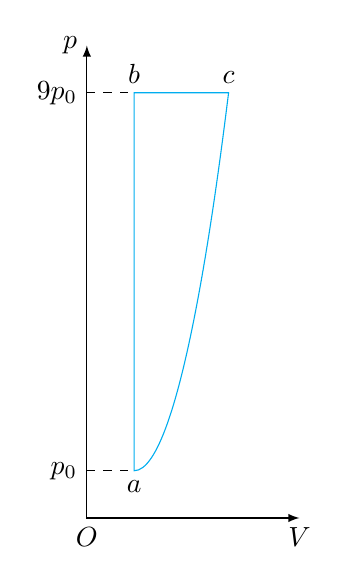
\begin{tikzpicture}[scale = 0.6]
            %画坐标轴
            \draw[latex-latex] (0, 10) -- (0, 0) -- (4.5, 0);
            \node[below] at (4.5,0) {$V$};
            \node[left ] at (0, 10) {$p$};
            \node[below] at (0, 0) {$O$};

            %画出虚线辅助线
            \draw[dashed] (0, 9) -- (1, 9);
            \draw[dashed] (0, 1) -- (1, 1);

            %画出p-V曲线
            \draw[cyan] (1,1) parabola (3,9) -- (1,9) -- (1,1) -- cycle;

            %标注出各个点
            \node[left ] at (0, 9) {$9p_0$};
            \node[left ] at (0, 1) {$p_0$};
            \node[below] at (1, 1) {$a$};
            \node[above] at (1, 9) {$b$};
            \node[above] at (3, 9) {$c$};
        \end{tikzpicture}
    \end{center}
\end{question}
\begin{solution}
    (1)对于 $a \to b$ 的等体过程,有$\frac{T_b}{p_b} = \dfrac{T_a}{p_a}$,则
    $$
        Q_{ab} = C_{V,\mathrm{m}}(T_b - T_a) = \frac{3}{2}R(9T_0 - T_0) = 12RT_0
    $$
    对于 $b \to c$ 的等压过程,有 $V_c = 3V_0$,$T_c = \dfrac{V_c}{V_b}T_b = 27T_0$,则
    $$
        Q_{bc} = C_{p,\mathrm{m}}(T_c - T_b) = \frac{5}{2}R(27T_0 - 9T_0) = 45RT_0
    $$
    对于 $c \to a$ 的多方过程,有$pV^{-2} = C$,多方指数为 $n=-2$,而多方过程的热容为
    $$
        C_{n,m} = C_{V,\mathrm{m}} \cdot \frac{\gamma - n}{1 - n} = \frac{11}{6}R
    $$
    于是得到
    $$
        Q_{ca} = C_{n,m}(T_a - T_c) = -47.7RT_0
    $$
    (2)这一循环的效率为
    $$
        \eta
        = \frac{|Q_{ab} + Q_{bc}| - |Q_{ca}|}{|Q_{ab} + Q_{bc}|}
        = \frac{12+45-47.7}{12+45}
        = 16.4\%
    $$
\end{solution}

\begin{question}{题目4.7.1}
    将热机与热泵组合在一起的暖气设备称为动力暧气设备,其中带动热泵的动力由热机燃烧燃料对外界做的功来提供. 热泵从天然蓄水池或从地下水取出热量,向温度较高的暖气系统的水供热同时,暖气系统的水又作为热机的冷却水. 若燃烧 $1 \,\si{kg}$ 燃料,锅炉能获得的热量为 $H$,锅炉、地下水、暖气系统的水的温度分别为 $210 \,\si{^\circ C}$,$15 \,\si{^\circ C}$,$60 \,\si{^\circ C}$. 设热机及热泵均是可逆卡诺机. 试问每燃烧 $1 \,\si{kg}$ 燃料,暖气系统所获得热量的理想数值(不计各种实际损)是多少?
\end{question}
\begin{solution}
    卡诺热机工作在锅炉和暖气系统之间,它先从锅炉获取热量 $H$,再做功 $W$ 驱动热泵,最后向暖气系统排放废热 $Q_1 = H - W$;而热泵工作于地下水和暖气系统之间,它被热机输出的功 $W$ 所驱动,从低温的地下水取热 $Q_2$ 并向暖气系统供热.

    热机工作在锅炉和暖气系统之间,根据卡诺热机效率 $\eta_\text{热}$ 的定义
    $$
        \eta_\text{热} = \frac{W}{H} = 1 - \frac{T_3}{T_1}
    $$
    导出热机用于驱动热泵的功 $W$
    $$
        W = \left(1-\frac{T_3}{T_1}\right) H
    $$
    热机做功后会继续向暖气排放废热
    $$
        Q_1 = H-W
        = H - \left(1 - \frac{T_3}{T_1} \right) H
        = \frac{T_3}{T_1}H
        \approx 0.69H
    $$
    热泵由热机所驱动,且热泵工作在地下水 $T_2$ 和暖气系统 $T_3$ 之间,那么根据热泵供热系数 $\varepsilon$ 的定义
    $$
        \varepsilon = \frac{Q}{W} = \frac{T_3}{T_3 - T_2}
    $$
    可以得到热泵从地下水取热 $Q_2$
    $$
        Q_2 = \frac{T_3}{T_3 - T_2} W
        = \left(\frac{T_3}{T_3 - T_2}\right) \left(1 - \frac{T_3}{T_1}\right) H
        \approx 2.30H
    $$
    最终暖气得到的热量 $Q_\text{暖气}$ 为热机排放的废热 $Q_1$ 和热泵从地下水抽取的热量 $Q_2$ 之和
    $$
        Q_\text{暖气} = Q_1 + Q_2
        = \frac{T_3}{T_1}H + \left(\frac{T_3}{T_3 - T_2}\right) \left(1 - \frac{T_3}{T_1}\right) H
        \approx 3.00H
    $$
    由此可见暖气最终得到的热量 $Q_\text{暖气}$ 约为锅炉燃烧产热 $H$ 的 3 倍.
\end{solution}
\section{热力学第二定律与熵}
\begin{question}{题目5.3.1}
    如图所示,$1 \,\si{mol}$ 氢气(理想气体)在 $1$ 点的状态参量为 $V_1 =0.02 \,\si{m^3}$,$T_1 =300 \,\si{K}$; 在 $3$ 点的状态参量为 $V_3 = 0.04 \,\si{m^3}$,$T_3 = 300 \,\si{K}$.图中 $1 \to 3$ 为等温线,$1 \to 4$ 为绝热线,$1 \to 2$ 和 $4 \to 3$ 均为等压线,$2 \to 3$等体线. 试分别用如下三条路径计算 $S_3-S_1$ :

    \begin{enumerate}
        \item[(1)] 路径 $1 \to 2 \to 3$
        \item[(2)] 路径 $1 \to 3$
        \item[(3)] 路径 $1 \to 4 \to 3$
    \end{enumerate}

    \begin{center}
        \begin{tikzpicture}[domain = 1:4]
            %画坐标轴
            \draw[latex-latex] (0,5) -- (0,0) -- (5,0);
            \node[left] at (0,5) {$p$};
            \node[below] at (5,0) {$V$};
            \node[below] at (0,0) {$O$};

            %画出1-2-3-4回路
            \draw[cyan] (1,4) parabola bend (2,1) (4,1) -- (4,4) -- (1,4) -- cycle;
            \draw[cyan] plot(\x, {4/\x} );

            %标注点
            \node [left ] at (1,4) {$1$};
            \node [right] at (4,4) {$2$};
            \node [below right] at (4,1) {$3$};
            \node [below left ] at (2,1) {$4$};

            %标注出箭头
            \draw[cyan, -latex] (2.5,4) -- (2.6,4);
            \draw[cyan, -latex] (4,2.5) -- (4,2.4);
            \draw[cyan, -latex] (2.5,1) -- (2.6,1);
        \end{tikzpicture}
    \end{center}
\end{question}

\begin{solution}
    (1) 路径 $1 \to 2$ 是等压过程,所以有 $T_2 = \dfrac{V_2}{V_1}T_1 = 600 \,\si{K}$ ,而路径 $2 \to 3$ 是等体过程,所以整个过程的熵变可以表示为
    $$
        S_3 - S_1
        = \int_{(1)}^{(2)} \frac{\mathrm{d}Q}{T} + \int_{(2)}^{(3)} \frac{\mathrm{d}Q}{T}
        = C_{p,\mathrm{m}}\int_{300}^{600}\frac{\mathrm{d}T}{T} + C_{V,\mathrm{m}}\int_{600}^{300}\frac{\mathrm{d}T}{T}
        = R\ln2
    $$
    (2) 路径 $1 \to 3$ 是等温过程,其熵变为
    $$
        S_3 - S_1 = \int_{(1)}^{(3)} \frac{\mathrm{d}Q}{T} = R\ln\frac{V_3}{V_2} = R\ln2
    $$
    (3) 路径 $1 \to 4$是绝热过程,满足
    $$
        T_1V_1^{\gamma-1} = T_4V_4^{\gamma-1}
    $$
    而路径 $4 \to 3$ 的等压过程满足
    $$
        \frac{T_4}{T_3} = \frac{V_4}{V_3}
    $$
    联立以上两式,将未知的 $V_4$ 用已知的 $V_3$ 代换
    $$
        T_4 = T_1 \left(\frac{V_1}{V_4}\right)^{\gamma-1}
        = T_1 \left(\frac{V_1T_3}{V_3T_4}\right)^{\gamma-1}
    $$
    分离 $T_4$ 后得到
    $$
        T_4^{\gamma} = T_1\left(\frac{V_1}{V_3}\right)^{\gamma-1}T_3^{\gamma-1}
    $$
    其中 $T_1 = T_3 = 300 \,\si{K}$,$\gamma = \dfrac{C_p}{C_V} = \dfrac{7}{5} $
    $$
        T_4
        = \sqrt[\gamma]{T_1\left(\frac{V_1}{V_3}\right)^{\gamma-1}T_3^{\gamma-1}}
        = \left(\frac{1}{2}\right)^{\frac{2}{7}} \times 300 \,\si{K}
    $$
    综上,路径 $1 \to 4 \to 3$ 过程的熵变可以表示为
    $$
        \begin{aligned}
            S_3 - S_1
             & = (S_4 - S_1) + (S_3-S_4)                                                                          \\
             & = 0 + \int_{T_4}^{T_3} \frac{\mathrm{d}Q}{T}                                                       \\
             & = C_{p,\mathrm{m}}\int_{T_4}^{T_3} \frac{\mathrm{d}T}{T}                                           \\
             & = \frac{7R}{2}\int_{\left(\frac{1}{2}\right)^{\frac{2}{7}} \times 300}^{300} \frac{\mathrm{d}T}{T} \\
             & = \frac{7R}{2} \cdot \ln\left(\frac{1}{2}\right)^{-\frac{2}{7}}                                    \\
             & = R \ln2
        \end{aligned}
    $$

\end{solution}

\begin{question}{题目5.3.3}
    水的比热容是 $4.18 \,\si{kJ \cdot kg^{-1} \cdot K^{-1}}$
    \begin{enumerate}
        \item[(1)] $1 \,\si{kg}$,$0^\circ C$ 的水与一个 $373 \,\si{K}$ 的大热源相接触,当水的温度到达 $373 \,\si{K}$ 时,水的熵改变多少?
        \item[(2)] 如果先将水与一个 $323 \,\si{K}$ 的大热源接触,然后再让它与一个 $373 \,\si{K}$ 的大热源接触,求整个系统的熵变.
        \item[(3)] 说明怎样才可使水从 $273 \,\si{K}$ 变到 $373 \,\si{K}$ 而整个系统的熵不变.
    \end{enumerate}
\end{question}
\begin{solution}
    (1)设水的初始温度为 $T_1$ , 水的最终温度为 $T_3$ ,水的定压比热容为 $c_p$,那么水的熵变可以表示为
    $$
        \Delta{S} = \int_{T_1}^{T_3} \frac{\mathrm{d}Q}{T}
        = mc_p\int_{T_1}^{T_3} \frac{\mathrm{d}T}{T}
        = mc_p\ln\frac{T_3}{T_1}
        = 1304.61 \,\si{J \cdot K^{-1}}
    $$
    (2)系统的总熵变应为两次水的熵变和两次热源的熵变之和,可以分别表示为
    $$
        \Delta{S}_{\text{水}}
        = mc_p\ln\frac{T_2}{T_1} + mc_p\ln\frac{T_3}{T_2}
        = mc_p\ln\frac{T_2T_3}{T_1T_2}
        = 1.30 \times 10^3 \,\si{J \cdot K^{-1}}
    $$
    $$
        \Delta{S}_{\text{热源}}
        = \frac{Q_2}{T_2} + \frac{Q_3}{T_3}
        = \frac{-mc_p(T_2-T_1)}{T_2} + \frac{-mc_p(T_3-T_2)}{T_3}
        = -1207.38 \,\si{J \cdot K^{-1}}
    $$
    $$
        \Delta{S} = \Delta{S}_{\text{水}} + \Delta{S}_{\text{热源}}
        \approx 97 \,\si{J \cdot K^{-1}}
    $$
    (3)我们注意到,中间温度热源的加入可以使得升温过程中系统的总熵变减少,所以只要不断地增加一系列温差无穷小中间热源,使得水的每一次升温的幅度都趋近于无穷小(即水的每一次升温都是可逆过程),最终就可以实现整个系统在升温过程中保持总熵不变.
\end{solution}

\begin{question}{题目5.3.5}
    有一热机循环,它在 $T - S$ 图上可表示为其半长轴和半短轴平行于 $T$ 轴和 $S$ 轴的椭圆,循环中熵的变化范围为从 $S_0$ 到 $3S_0$,$T$的变化范围为 $T_0$ 到 $3T_0$,试求该热机的效率.
\end{question}
\begin{solution}
    依题意画出示意图
    \begin{center}
        \begin{tikzpicture}
            %画坐标轴
            \draw[latex-latex] (0,6.5) -- (0,0) -- (3.5,0);
            \node[below] at (3.5, 0) {$S$};
            \node[left ] at (0, 6.5) {$T$};
            \node[below] at (0,0) {$O$};

            %标注点
            \node [right] at (3, 4) {$1$};
            \node [below] at (2, 2) {$2$};
            \node [left ] at (1, 4) {$3$};
            \node [above] at (2, 6) {$4$};
            \node [left ] at (0, 2) {$T_0$};
            \node [left ] at (0, 6) {$3T_0$};
            \node [below] at (1, 0) {$S_0$};
            \node [below] at (3, 0) {$3S_0$};

            %画出虚线
            \draw [dashed] (3, 4) -- (3, 0); %1的垂线
            \draw [dashed] (2, 2) -- (0, 2); %2的垂线
            \draw [dashed] (1, 4) -- (1, 0); %3的垂线
            \draw [dashed] (2, 6) -- (0, 6); %4的垂线

            %画出椭圆
            \draw [cyan] (2,4) ellipse (1 and 2);
        \end{tikzpicture}
    \end{center}
    在 $T - S$ 图上顺时针循环所围成的面积就是热机对外所做的功 $W$ (椭圆的面积为 $S = \pi a b$)
    $$
        W = \pi T_0 S_0
    $$
    路径 $3 \to 4 \to 1$ 是熵增加的过程,它所吸收的热量 $Q$ 可以表示为曲线$3 \to 4 \to 1$ 所围的面积
    $$
        Q = \frac{\pi T_0 S_0}{2} + 2T_0 \cdot 2S_0
        = \left(\frac{\pi}{2} + 4\right) T_0 S_0
    $$
    所以热机的效率 $\eta$ 可以表示为
    $$
        \eta = \frac{W}{Q}
        = \frac{\pi T_0S_0}{\left(\frac{\pi}{2} + 4\right)T_0S_0}
        = \frac{2\pi}{\pi+8}
    $$
\end{solution}

\begin{question}{题目5.3.6}
    理想气体经历一正向可逆循环,其循环过程在 $T-S$ 图上表示为从 $300 \,\si{K}$,$1 \times 10^6 \,\si{J \cdot K^{-1}}$ 的状态等温地变为 $300 \,\si{K}$,$5 \times 10^5 \,\si{J \cdot K^{-1}}$ 的状态,然后等熵地变为 $400 \,\si{K}$,$5 \times 10^5 \,\si{J \cdot K^{-1}}$ 的状态,最后按一条直线变回到 $300 \,\si{K}$,$1 \times 10^6 \,\si{J \cdot K^{-1}}$ 的状态.试求循环效率及它对外所做的功.
    \begin{center}
        \begin{tikzpicture}[scale = 0.8]
            %画坐标轴和原点
            \draw[latex-latex] (3, 5) -- (3, 0) -- (11, 0);
            \node[left ] at (3, 5) {$T / (\mathrm{K})$};
            \node[below right] at (11,0) {$S / \mathrm{(kJ \cdot K^{-1})}$};
            \node[below] at (3, 0) {$O$};

            %画虚线
            \draw[dashed] (3, 3) -- (5,3) -- (5,0);
            \draw[dashed] (3, 4) -- (5, 4);
            \draw[dashed] (10, 3) -- (10,0);

            %画循环箭头
            \draw[cyan] (5, 3) -- (5, 4) -- (10, 3) --cycle;
            \draw[-latex, cyan] (10,3) -- (7.5, 3.0); % 1 -> 2
            \draw[-latex, cyan] (5, 3) -- (5.0, 3.5); % 2 -> 3
            \draw[-latex, cyan] (5, 4) -- (7.5, 3.5); % 3 -> 1

            %标注7个参考点
            \node[left ] at (3, 4) {$400$};
            \node[left ] at (3, 3) {$300$};
            \node[below] at (5, 0) {$500$};
            \node[below] at (10,0) {$1000$};
            \node[below right] at (10,3) {$1$};
            \node[below left] at (5, 3) {$2$};
            \node[above left] at (5, 4) {$3$};
        \end{tikzpicture}
    \end{center}
\end{question}
\begin{solution}
    路径 $1 \to 2$ 是等温过程,熵是减小的,释放的热量为
    $$
        Q_\text{放} = T_1(S_1-S_2)
    $$
    路径 $2 \to 3$ 是等熵过程,是绝热的,所以
    $$
        Q = 0
    $$
    路径 $3 \to 1$ 过程熵增,它吸收的热量是曲线下的面积
    $$
        Q_\text{吸}
        = \int_{S_1}^{S_2} T \,\mathrm{d}S
        = 1.75 \times 10^8 \,\si{J}
    $$
    而系统在整个循环过程中对外做功为图中三角形所围的面积,即
    $$
        W = 2.5 \times 10^7 \,\si{J}
    $$
    所以循环的效率 $\eta$ 为
    $$
        \eta = \frac{W}{Q_\text{吸}}
        = \frac{2.5 \times 10^7}{1.75 \times 10^8}
        = \frac{1}{7}
    $$
\end{solution}

\begin{question}{题目5.3.8}
    在一绝热容器中,质量为 $m$ 、温度为 $T_1$ 的液体和相同质量但温度为 $T_2$ 的同种液体在一定压强下混合后达到新的平衡态,求系统从初态变到终态熵的变化,并说明熵是增加的,设已知液体定压比热容为常量 $c_p$. (注意:液体的体膨胀系数是非常小的.)
\end{question}
\begin{solution}
    由于容器绝热,所以混合前后液体的总内能保持不变. 我们不妨设混合后的平衡温度为$T$,则
    $$
        mc_pT_1 + mc_pT_2 = 2mc_pT
    $$
    解得
    $$
        T = \frac{T_1 + T_2}{2}
    $$
    混合前后两份液体的熵变分别为
    $$
        \Delta{S_1} = \int_{T_1}^{T} \frac{\mathrm{d}Q}{T}
        = mc_p\int_{T_1}^{T} \frac{\mathrm{d}T}{T}
        = mc_p\ln\frac{T}{T_1},
    $$
    $$
        \Delta{S_2} = \int_{T_2}^{T} \frac{\mathrm{d}Q}{T}
        = mc_p\int_{T_2}^{T} \frac{\mathrm{d}T}{T}
        = mc_p\ln\frac{T}{T_2},
    $$
    系统总熵变为二者之和
    $$
        \Delta{S} = \Delta{S_1} + \Delta{S_2}
        = mc_p\ln\frac{T^2}{T_1T_2}
        = mc_p\ln\left[\frac{(T_1 + T_2)^2}{4T_1T_4}\right]
    $$
    考虑到对于互不相等的 $T_1>0$ 和 $T_2>0$ ,有不等式
    $$
        (T_1+T_2)^2 > 4T_1T_2
        \implies
        \frac{(T_1+T_2)^2}{4T_1T_2} > 1
    $$
    恒成立,所以 $\Delta{S} > 0$ 成立,即总熵是增加的.
\end{solution}

\begin{question}{题目5.3.9}
    某热力学系统从状态 $1$ 变化到状态 $2$ . 已经知道状态 $2$ 的热力学概率是状态$1$ 的热力学概率的 $2$ 倍,试确定系统熵的增量.
\end{question}
\begin{solution}
    考虑到玻尔兹曼关系 $S = k \ln{W}$,设 $W_2 = 2W_1$ 所以熵增为
    $$
        \Delta{S} = k\ln{W_2} - k\ln{W_1} = k\ln{2} =9.57 \times 10 ^{-24} \,\si{J \cdot K^{-1}}
    $$
\end{solution}

\end{document}